\textbf{Indeks} to struktura danych, w przechowywane są adresy fizyczne krotek oraz atrybuty, względem których sortowane są krotki. Takie atrybuty nazywa się kluczami wyszukiwania, ale wcale nie muszą to być klucze relacji.
Indeksy powinny przede wszystkim umożliwiać szybkie wyszukiwanie, dodawanie oraz usuwanie elementów.

\subsection{Implementacje indeksów}
\subsubsection*{B+-drzewo}
To struktura danych do przechowywania danych posortowanych według pewnego klucza. Umożliwia operacje wyszukiwania, dostępu sekwencyjnego, wstawiania i usuwania w czasie \( \bigO(\log_{\frac{M}{2}} N) \).
Jest implementowana jako ukorzenione, zbalansowane drzewo \( M \)-arne, w którym każdy wierzchołek poza korzeniem ma \( k \) kluczy, gdzie \( \frac{M}{2} - 1 \leq k \leq M - 1 \),
a węzeł wewnętrzny o \( k \) kluczach ma \( k+1 \) potomków. Węzły wewnętrzne przechowują tablice z parami <node*, key>, a liście wartości (krotki lub adresy) <value, key>.
Ogólnie im wolniejsza jest pamięć, tym większy jest optymalny rozmiar węzła.
Najszybciej można zbudować B+-drzewo, sortując klucze, a potem budując indeks od dołu (bulk loading).
\begin{figure}[h!]
    \centering
    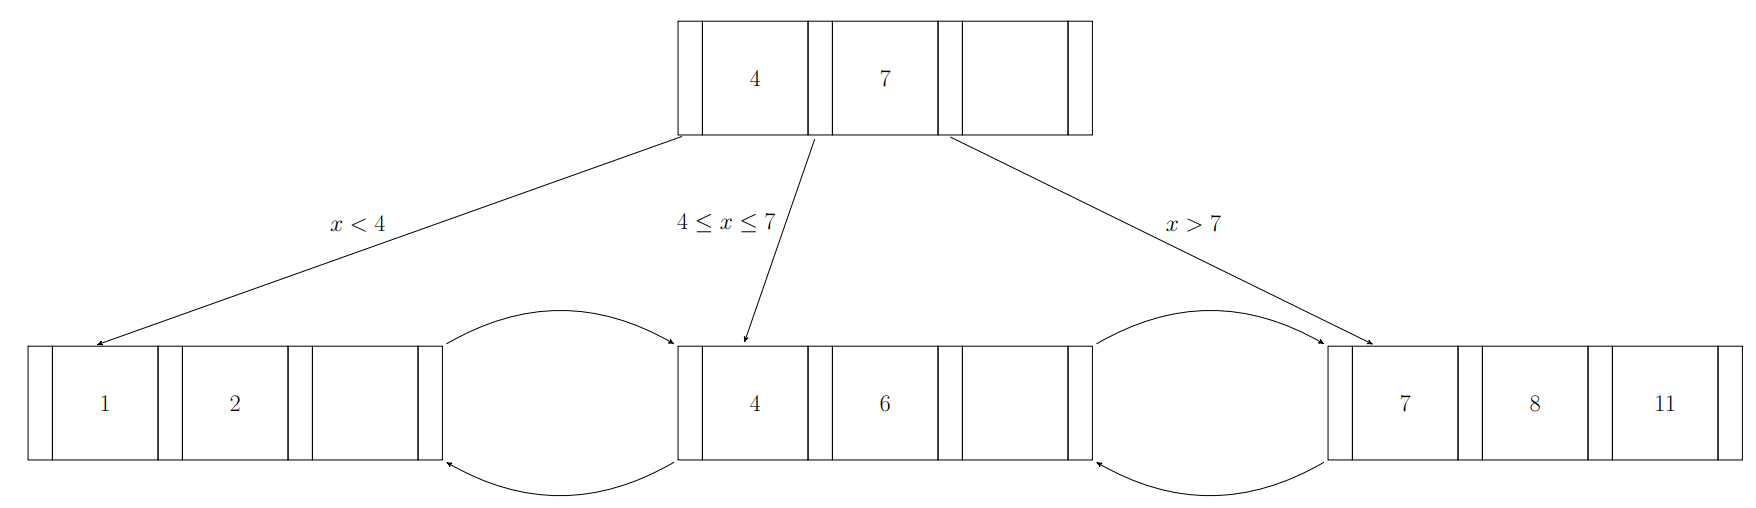
\includegraphics[width=0.75\linewidth]{chapters/id/indeksy/b_tree}
    \caption{Schemat B+-drzewa}
\end{figure}

Zalety B+-drzew:
\begin{itemize}
    \item mała liczba odczytów z dysku
    \item efektywne na każdym poziomie hierarchii pamięci
    \item względnie efektywne i dla dostępu swobodnego, i sekwencyjnego
    \item efektywne dla różnych typów danych
\end{itemize}
Wada: rozmiar rośnie liniowo
\href{https://www.cs.usfca.edu/~galles/visualization/BPlusTree.html}{wizualizacja \fcTree}

\subsubsection*{Indeks pokrywający}
To rodzaj indeksu, który przechowuje wartości niektórych atrybutów, względem których nie jest tworzony indeks.

\subsubsection*{Indeks haszowy}
W przeciwieństwie do B+-drzew, rozmiar indeksów haszowych rośnie skokowo, gdy przydzielana jest dodatkowa pamięć dla nowych kubełków.
Rozmiar nie jest zależny od rozmiaru haszowanych wartości.

\subsubsection*{Indeks bitmapowy}
Ten rodzaj indeksu koduje w mapach bitowych wartości krotek z wybranej kolumny. Pozwala sprowadzić niektóre zapytania do operacji bitowych.

\subsection{Kiedy warto korzystać z indeksów?}
Domyślnie dla każdej tabeli tworzony jest indeks odpowiadający kluczowi głównemu oraz każemu unikalnemu atrybutowi.
Im więcej indeksów, tym szybsze jest wyszukiwanie, ale też tym więcej miejsca zajmuje baza oraz czas synchronizacji i planowania wykonania zapytania jest dłuższy.
Kiedy więc warto tworzyć dodatkowe indeksy?
\begin{itemize}
    \item zgrupowane (dane w kolejności jak na stronach):
    \begin{itemize}
        \item do operacji na zakresach
        \item do pobierania danych w określonym porządku
        \item do zapytań na wielu kolumnach
        \item do dodawania nowych wierszy
    \end{itemize}
    Efektywne, kiedy wartości są krótkie, rzadko się powtarzają i są rzadko zmieniane.
    \item częściowy (na wybranych wartościach atrybutu)
    \begin{itemize}
        \item do zapytań działających tylko na podzbiorze krotek
    \end{itemize}
    \item haszowany
    \begin{itemize}
        \item do zapytań równościowych
    \end{itemize}
    \item bitmapowy
    \begin{itemize}
        \item dla atrybutów o niewielkiej dziedzinie
    \end{itemize}
    \item B+-drzewa
    \begin{itemize}
        \item do zapytań równościowych i na zakresach
    \end{itemize}
\end{itemize}

Indeksy mogą działać wolniej kiedy:
\begin{itemize}
    \item zapytanie wymaga przeskanowania dużej części tabeli
    \item dane są często modyfikowane
\end{itemize}
